\section{Testing Results}
In this section, we test the running time of insertion, deletion and searching. We use \texttt{time()} function in C standard library to record the total time of $N$ operations (insertion/deletion/search). For small $N$, the running time is too short (less than 1 ms), we make several iterations of the same operations and compute the average time.\par 
As insertion/deletion will modify the skip list, the size of the skip list will change after each operation. Thus, we only record the total running time of $N$ insertions/deletions, instead of dividing $N$ to get the average time per operation (which is meaningless because the size of the skip list isn't fixed). But for searching, the size of the skip list doesn't change after each operation, so we can divide $N$ to get the average time per operation.
\subsection{Insertion}
In this test, we insert $N$ values from $0$ to $N-1$ into a skip list with $Max\_level=32$ in an order of
\begin{itemize}
    \item Increasing, i.e. $0,1,2,\ldots,N-1$
    \item Decreasing, i.e. $N-1,N-2,\ldots,1$
    \item Random
\end{itemize}
And we record the total time of $N$ insertions. The result is as follows:
\begin{figure}[H]
    \centering
    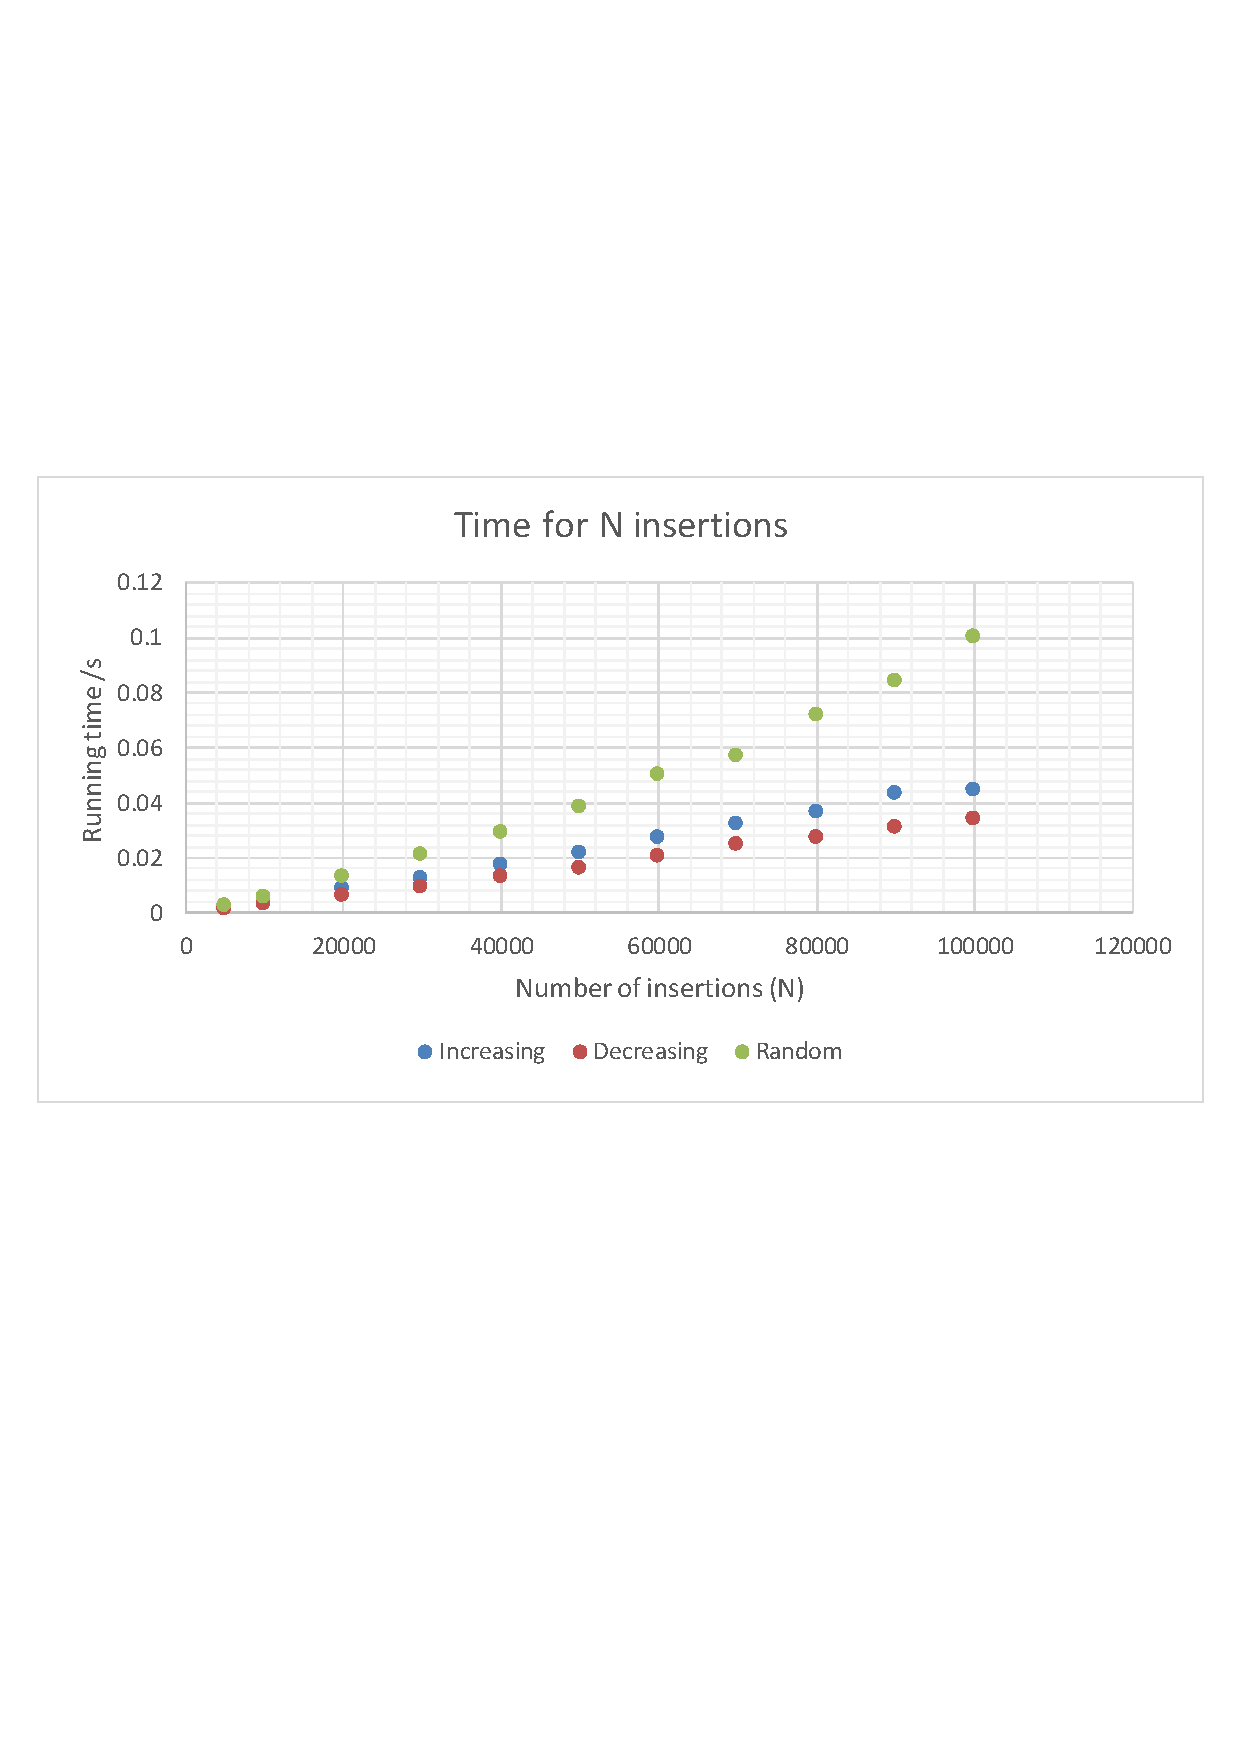
\includegraphics[width=\textwidth]{testing_results/insert.pdf}
    \caption{Running time for 3 insert orders}
\end{figure}

\subsection{Deletion}
We first create a skip list with $Max\_level=32$ and insert $N$ values from $0$ to $N-1$ into it. Then, we delete the values in an order of
\begin{itemize}
    \item Increasing, i.e. $0,1,2,\ldots,N-1$
    \item Decreasing, i.e. $N-1,N-2,\ldots,1$
    \item Random
\end{itemize}
We use the same method as we did in the insertion test to record the total time of $N$ deletions. The result is as follows:
\begin{figure}[H]
    \centering
    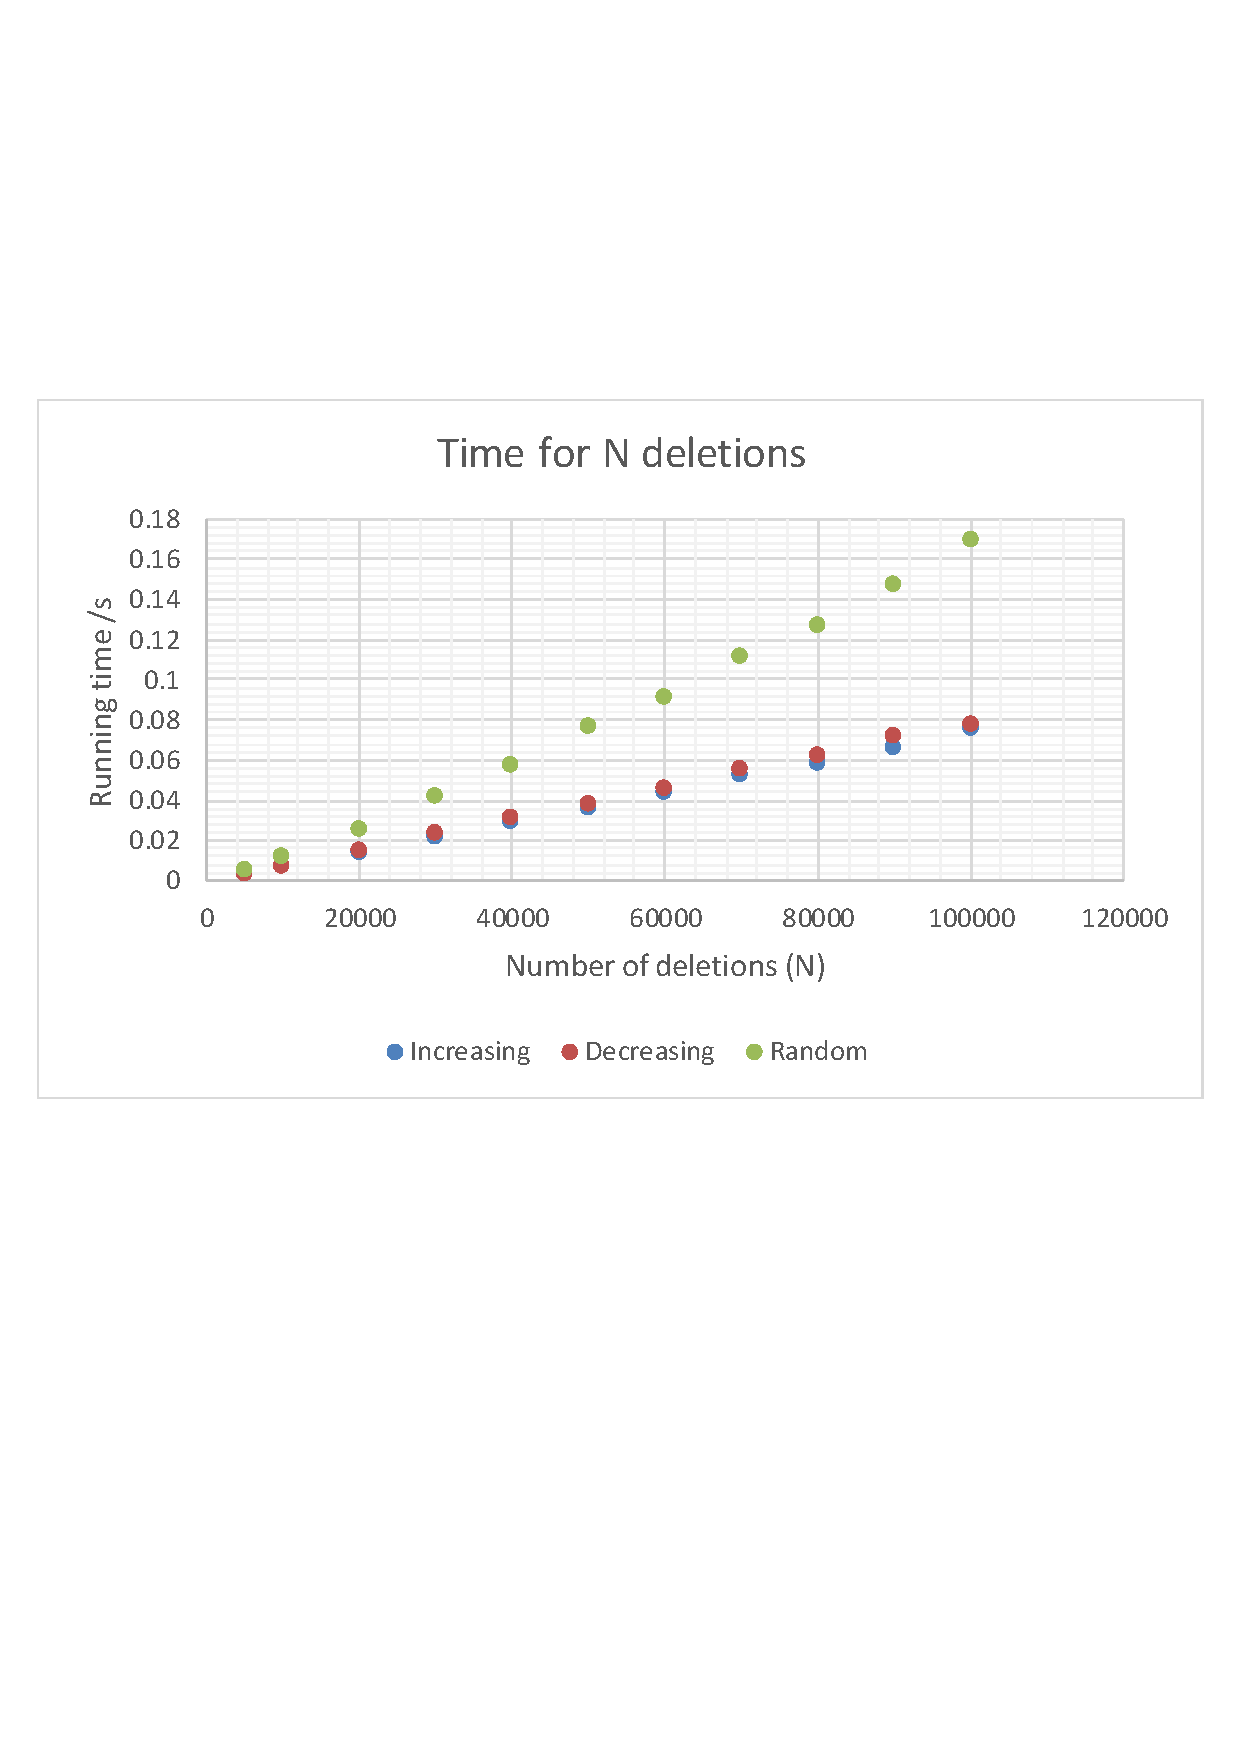
\includegraphics[width=\textwidth]{testing_results/delete.pdf}
    \caption{Running time for 3 delete orders}
\end{figure}

\subsection{Search}
Finally, we test the time of the find operation.\par
We first create a skip list with $Max\_level=32$ and insert $N$ values from $0$ to $N-1$ into it. Then, we find a random value between $[0, N)$ from the skip list for $N$ times. The average time per searching is $\frac{\text{total time}}{N}$. The result is as follows:
\begin{figure}[H]
    \centering
    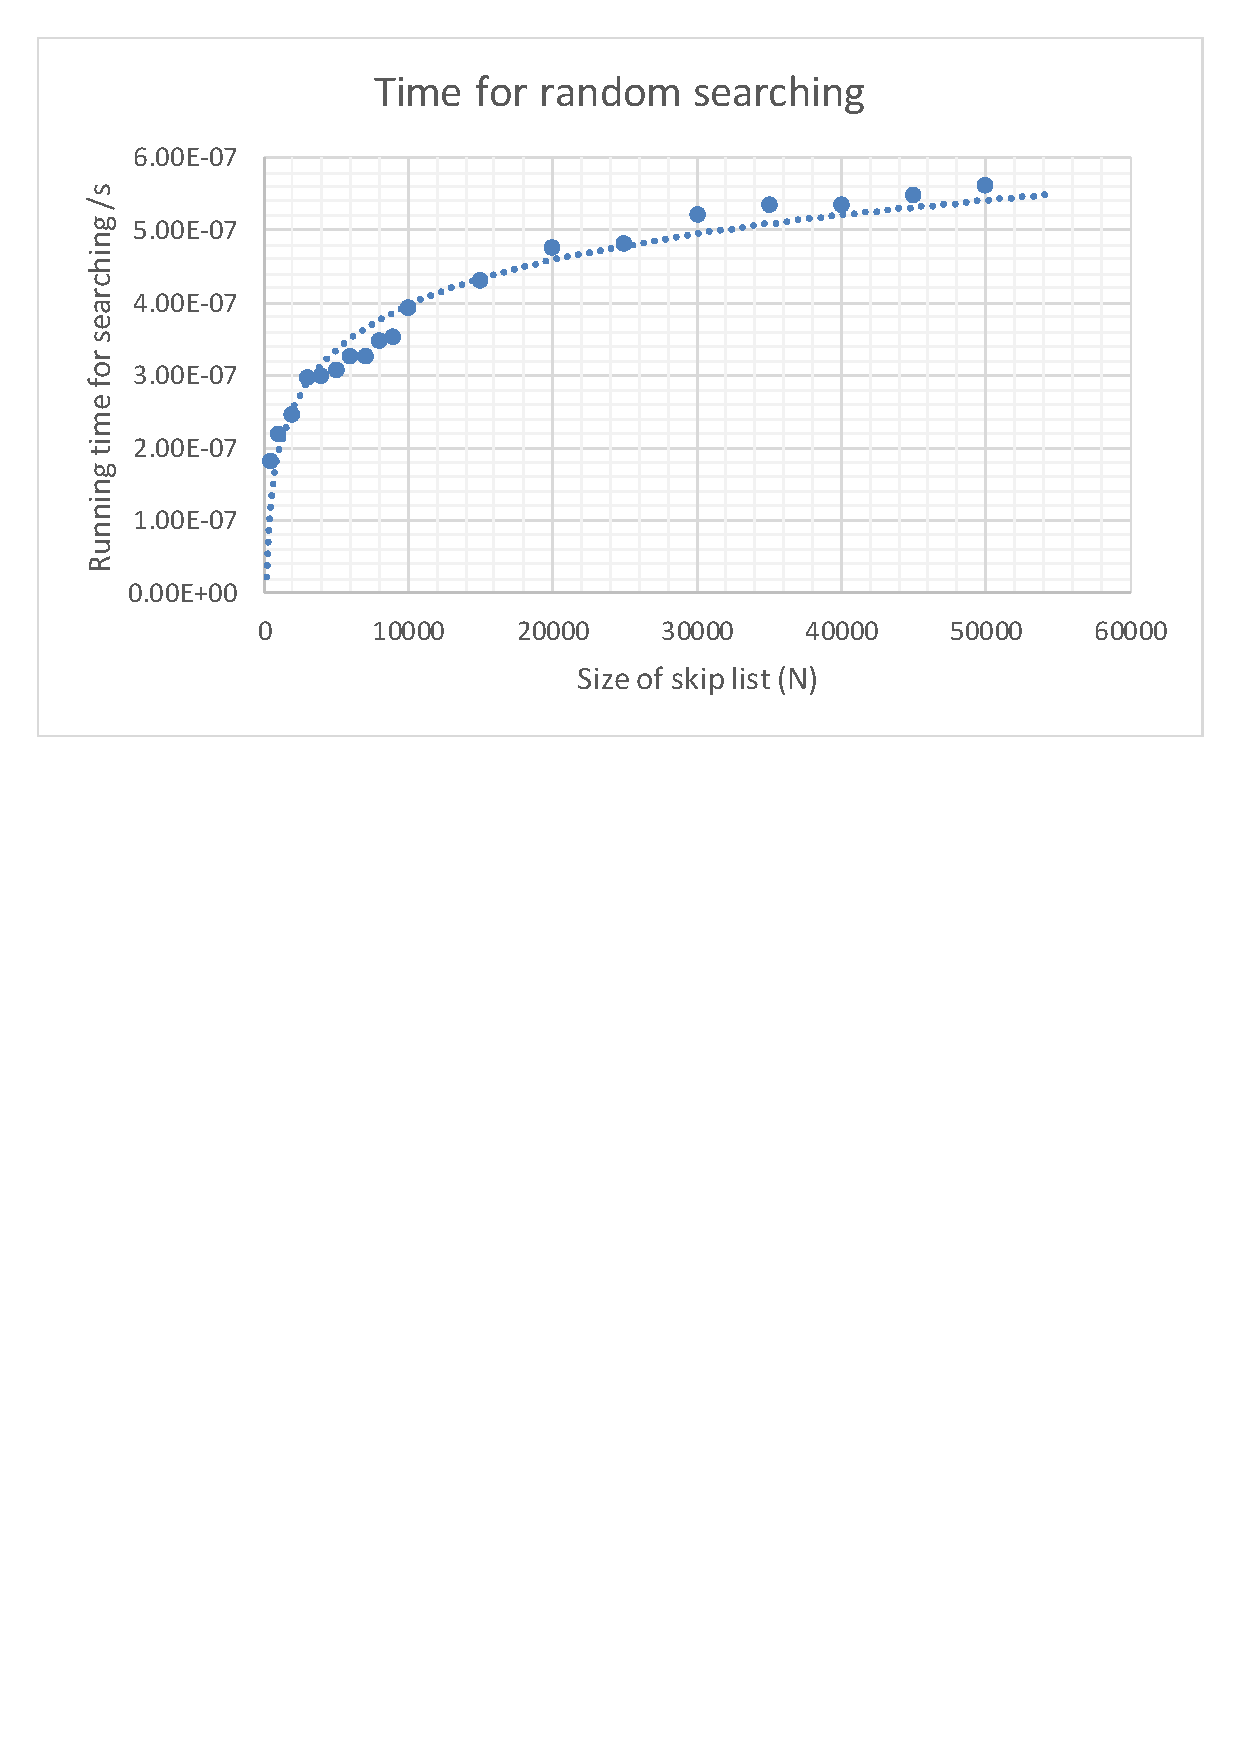
\includegraphics[width=\textwidth]{testing_results/search.pdf}
    \caption{Running time for searching}
\end{figure}
From the figure, we observe that the time complexity of finding seems to be $O(\log{N})$.